\documentclass[a4paper,11pt]{article}
\usepackage{graphicx}

\usepackage{microtype}

\usepackage[
backend=biber,
style=ieee,
]{biblatex}

\usepackage[margin=1in]{geometry}

\usepackage{fontspec}
\setmainfont{Times New Roman}

\addbibresource{references.bib}

\title{WASP Software Engineering}
\author{Bj\"orn Wehlin}
\date{\today}

\begin{document}

\maketitle

\section{Introduction}

I'm a PhD student in the Topological Data Analysis group at the KTH Mathematics department. I do both applied and theoretical work. On the applied side, I have ongoing work on a variety of topics, including criminology \cite{wehlin2025poznan}, materials science (in which I have also worked prior to starting the PhD, \cite{cybart2015nano}), and medical imaging. For these, we try to make statistical conclusions from often very noisy data, using features derived from algebraic topology (persistent homology, etc.). On the theoretical side, I'm studying the geometry/topology of point processes, and discrete geometry.

In addition to this, I'm also the originator and lead maintainer of the open source project \emph{stablebear} (\url{https://www.stablebear.org}) \cite{stablebear}, which is a Python/C++ package for working with large-scale topological data analysis, both on CPU and GPU.

\section{Lecture Principles}

\subsection{Groups and Creativity}

In one of the lectures \cite{feldt2026agentic}, it is discussed how agentic systems will impact groups. One of the points that is brought forward, from a paper by Doshi and Hauser \cite{doshi2024generative}, is that AI can raise creativity among individuals but bring down collective diversity. As an example, they show that AI-assisted creative writing can lead to stories with more ideas, but that the stories become similar between writers.

At the moment, in my research, I'm trying to solve a problem in discrete geometry by using LLMs. Many mathematical conjectures have been solved this way recently \cite{vibemathed}, although progress seems to have stalled a bit lately. I will say I sense a bit of both of the conclusions from \cite{doshi2024generative} discussed above. 

On the positive side, I have been able to expose the problem to a large number of ideas from various fields, many of which I have not been familiar with. In a traditional research setting, in order to try these ideas, I would have to spend months or years getting acquainted with some of these fields and their methods, just to see a majority of the ideas fail in the end. With the LLM, I'm able to have \emph{it} try these ideas without my having to become an expert first.

On the other hand, I find that the LLM is quite poor at coming up with original ideas by itself (as one may reasonably expect). For example, much of what we are doing relies on coming up with certain decompositions of various spaces. Here, we as human mathematicians have had to play the lead role and feed these ideas to the LLM as opposed to the LLM proposing them by itself. As such, the LLM can be thought of more as a tool as opposed to a fully autonomous mathematician.

\subsection{Random testing}

In the lecture on Quality Assurance \cite{feldt2026qa}, randomized testing is highlighed as a strategy for creating test cases. This is certainly something that could be added to \emph{stablebear}. In fact, it has been considered in the past, but has not been worked on because other items have had higher priority. We have also considered adding \emph{mutation testing} as it can help identify where we need to add test coverage to ensure that the implementations of mathematical algorithms are correct. 

In our setting, boundary value/edge case testing, which is also mentioned in \cite{feldt2026qa}, is very important, and we do spend time working on test cases for this.

\section{Guest lecture principles}

\subsection{RE4AI Research:
Prioritization of Software Qualities}

In Julian Frattini's guest lecture \cite{frattini2026agentic}, it is argued that how important certain qualities are differes between traditional software engineering and AI systems engineering (this in turn from \cite{Habibullah2023Non}). For example, usability is seen as less important in an AI system, whereas maintainability and accuracy become more important.

The part about accuracy is, in my view, a bit questionable. In \cite{Habibullah2023Non}, accuracy is defined as ``the number of correctly predicted data points out of all the data points.'' It is true that this type of relationship not typically a concern in most traditional software, as \cite{Habibullah2023Non} points out, but I think this fairly limited view of ``accuracy'' risks creating a view that \emph{correctness} is not a concern of traditional software. As a, perhaps tongue-in-cheek, example: an elevator control system that does not stop the elevator on the correct floor (or worse, stops the elevator in-between floors) certainly would not pass even the most basic system acceptance test by a customer.

Even in the machine learning context, I find accuracy to be a fairly limiting metric. For example, much of my work incorporates \emph{unsupervised learning}. In this context, there are no labels to compare against, and thus no accuracy in the sense of \cite{Habibullah2023Non, frattini2026agentic}.

I would offer that \emph{correctness} is a concern of equal importance between both AI and traditional software systems.

\subsection{Semi-executable stack: A diagnostic map of SE}

In Per Lenberg's guest lecture \cite{lenberg2026importance}, a comparison between pre-AI and post-AI work is made for several components of the software lifecycle.

Some of these components, code perhaps most prominently, can be more or less completely replaced by gen-AI. However, the human workflows, such as ticket management, meetings, and so on, probably will see less impact. Lenberg lists, e.g., AI tool use and human-agent loops as AI mediation for this topic \cite{lenberg2026importance}. This will likely happen more and more. For example, AI agents surely are capable of filing an understandable ticket from underspecified or ill-explained human input, at least with iteration. Likewise, AI can be used to understand already-filed tickets.

In the \emph{stablebear} project, we have used coding agents to go through the codebase and documentation automatically, and file issues with automatic prioritization, etc.. The prioritization is not always correct, but at least it can serve as a first filter. We have found several real issues from doing this, but we are now also inundated by AI-generated fixes for these issues that must be reviewed by a human. At the moment, I don't have a good solution for this problem, and, more generally, it is a growing problem in the software community at large.

\section{Data scientists, software engineers, and AI engineers}

If I were to give a short overview of Chapters 1 and 2 in \cite{kastner2025machine}, it is the following. Data science in industry differs from data science in the lab in that, while in the lab, models are usually developed as ``one-offs,'' pushing specific metrics, whereas in the ``real-world'' setting, a much broader infrastructure is needed to maintain a model over time. K\"{a}stner dubs this shift of mindset as having a ``system-level view'' \cite{kastner2025machine}.

From a software engineering point-of-view, this type of approach is already very common with continuous integration and delivery\footnote{The present author feels the need to express his distaste with continuous delivery as a concept! Continuous integration is perfectly reasonable, though, and should most definitely be used as much as possible.} (CI/CD). When a change to a software system is proposed (typically via a pull request or similar mechanism), a continuous integration pipeline builds the application/system with the proposed change, and, at minimum, runs through one or several test suites. Continuous integration pipelines can be significantly expanded in scope, with static and runtime analysis (including memory, etc., checking), coverage reporting, and so on. In the best of worlds, after such a pipeline has finished, human reviewer(s) give feedback on the change before it goes into production, and if changes need to be made, the process moves back to an earlier state. Nowadays, AI tools see increasing usage for both feedback and other uses. For an example of a CI pipeline, see Figure~\ref{fig:ci}.

\begin{figure}[t]
    \centering
    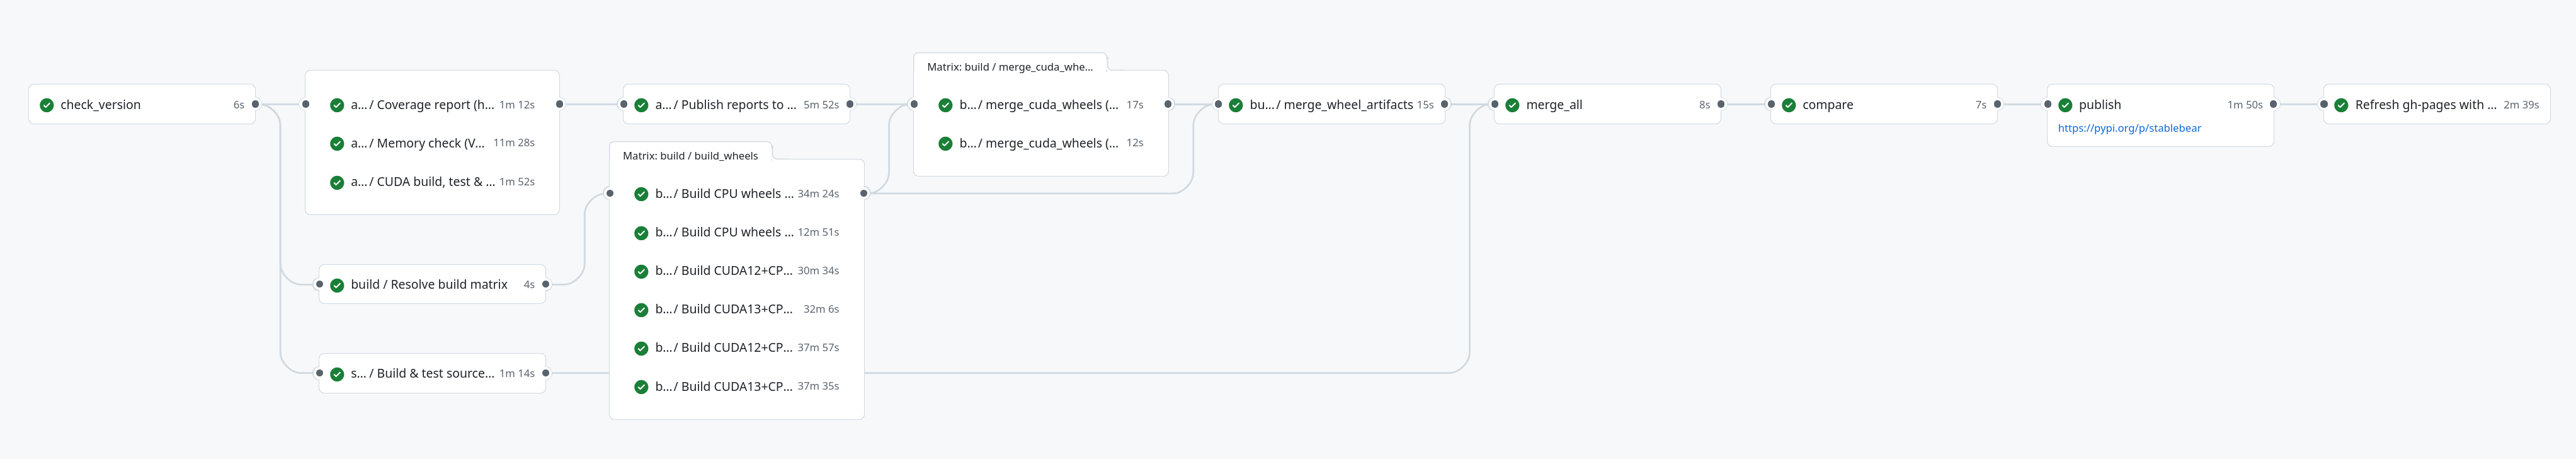
\includegraphics[width=\linewidth]{stablebear-ci.png}
    \caption{An overview of the release CI pipeline used in the \emph{stablebear} project. First, the proposed version number is checked against the PyPI repository (the build only proceeds if the version number is not already in use). Then, parallel streams are used to build and test the packages on the various supported platforms, and the CUDA build (this runs on a non-cloud machine since a physical GPU is required, and this is not provided for free by GitHub), which includes coverage reporting and memory checking. Next, all artifacts are merged into one package for later upload to PyPI. Then, a comparison step checks that all packages contain the correct contents, including licensing information and runtime libraries (where appropriate). Finally, a publishing step, which is gated by a manual approval, uploads the new release to the PyPI repository and creates a version tag in the project's Git repository.}
    \label{fig:ci}
\end{figure}

K\"{a}stner argues that a similar approach should be used also in a machine learning context. However, difficulties in developing, for example, unit tests is noted, due to the ``black-box'' nature of machine learning models \cite{kastner2025machine}. It is also argued that machine learning projects have challenges that differ from traditional software engineering. For example, this includes data drift that must be managed over time \cite{kastner2025machine}.

In my own view, software engineers and data scientists will continue to exist as separate roles. The former simply for the fact that a lot of software simply does not need an advanced understanding of statistics or mathematics. That said, software engineers certainly can learn from data scientists, particularly in the domain of randomized testing, as well as data presentation from test runs, etc.. For data scientists, it is less clear that they can remain completely within their own domain. Some level of software engineering skills is certainly needed for all practitioners of machine learning if these data scientists are to have any hope of implementing anything. I'm not convinced, though, that all data scientists have to become \emph{bona fide} software engineers in addition to their own expertise. In fact, there is a risk in attempting this as it steals time that can be used to improve on modeling, etc..

When it comes to coding agents, there are some good news, at the very least. These systems can explain to software engineers how to improve their testing, etc., whereas for data scientists, the AI agents can help with setting up CI pipelines (also helpful for software engineers!) and support quick iteration on models.

\section{Paper Analysis}

\subsection{Herbold et al. (2024): Legal aspects for software developers interested in generative AI applications}

As my first paper, I chose \cite{herbold2024legal} \emph{(full paper from CAIN 2026)}, which concerns the legal aspects of both data and models in the context of generative AI. There are two core issues at play: 1) the rights of individuals and copyright holders whose personal information and licensed works, respectively, may be part of training data, and 2) licensing implications for model developers and model consumers\footnote{By model consumers, I primarily mean organizations that access a model via an API to enable functionality in their own products or services.}. The paper provides an overview guide to some of the key legislation and (sparse) legal precedent in these areas for both research and industry practitioners.

On the level of personal information, legislation such as GDPR (EU General Data Protection Regulation) and CCPA (California Consumer Privacy Act) provide key provisions, such as the ``right to be forgotten'' (in the case of GDPR). For conventional databases it is essentially clear how to, although burdensome, for organizations to comply with the law. However, for data that get ``baked into'' the model weights, the situation is less clear. This is pointed out in \cite{herbold2024legal}, although the observation has been well-known for some time. 

Beyond personal information, the paper discusses the issue of copyrighted information entering the training data. It appears likely that as long as the model doesn't memorize a copyrighted work and is able to reproduce it, its inclusion in the training data would fall under fair use. However, it is hard, if not impossible, to ensure that such remembrance does not occur. This issue is discussed also in the context of personal information, but there the issue of filtering out such information is somewhat paradoxical as it may require another AI model to identify where any given person's information may be present, meaning that that model may require to have access to the personal information we are trying to filter out. I will note, however, that developers of generative AI models are not the only entities that must deal with this problem. Any organization that deals with private information must comply with the relevant data protection regulations. These entities are not allowed to hide behind an argument of ``we have too much data to filter manually,'' so it is unclear why generative AI companies are seemingly allowed to do so.

On the other hand, for model consumers, there are issues such as model licensing, etc., to take into account. The paper makes an argument that it is unclear whether models are copyrightable since their computed weights are not necessarily the process of human creativity. However, here I would interject that one could make the model architecture and surrounding ``plumbing'' the intellectual property rather than the model weights themselves.

My own research does not include any personal information as part of the data, and I am not training generative models on existing copyrighted data. I am however a consumer of generative AI tools for software engineering and research. 

From my use so far, I noticed one thing in the research context that is especially troubling: the models are quite good at describing methods from literature, but they are quite bad at citing sources when doing so. As such, while LLMs can be a great tool for finding methods and approaches that can be incorporated in one's research, one has to be careful to identify information that may not be novel and then look for relevant sources. Often, as a first step, one can ask follow-up questions to the LLM about where the information comes from, but manual searches may be necessary as well.

\subsection{Zheng et al. (2026): AI co-mathematician: Accelerating
mathematicians with agentic AI}

For my second paper, I chose \cite{zheng2026ai}. This is a paper out of Google DeepMind that discusses the \emph{AI co-mathematician}, which is an agentic, model-agnostic, system for mathematics research. 

The paper describes some design principles that are specific to mathematics and which may be missed by off-the-shelf coding agents. For example, this includes iterative refinement of ideas, production of mathematical artifacts in formats that are understandable by humans, management of cognitive load through progressive disclosure, and management of uncertainty \cite{zheng2026ai}.

The authors also present several case studies where mathematicians were given access to the (currently closed-access) tool and attempted to use it to solve problems within their respective areas.

As I have mentioned earlier, I am working on a discrete geometry problem using LLMs. More specifically, I am using coding agents such as Claude Code and OpenAI Codex for this purpose. Having also used these tools to develop my library \emph{stablebear}, it is clear that there are both differences and similarities between using coding agents for mathematics research and software engineering.

The similarities range from setting up and maintaining testing infrastructure to writing small falsification scripts. The coding agents can deal with both problems quite well since they were made for coding. They are even quite capable at writing formal verification code in Lean \cite{lean}.

However, perhaps due to how I have structured my workflow, the coding agents tend to create large text files containing mathematical reasoning (at the moment, the agents have produced over 260,000 lines of such text in my project, and I am now in the process of migrating the project into a ``theorem database'' to see if this makes the project more manageable and token-efficient).

Next, coding agents, from my own experience, and from reading various posts online, appear to have a tendency to overengineer. For mathematics, anecdotally, this behavior seems to be present as well (attempting overly complicated approaches, for example). But perhaps a more pressing issue is the tendency to end up in seemingly endless ``lemma pits.'' That is, the agent ``thinks'' that it is just one lemma away from proving the needed theorem, but then it discovers that it needs to prove another lemma to get to the first lemma, and then yet another lemma emerges, and so on and so forth. This concern is mirrored in \cite{zheng2026ai} in that the authors experience: ``Consequently, there is always a significant risk that
the model encounters an unplanned-for difficulty [...] It is clear from our experiences that current models’ judgment on what
to do in such cases is far behind human capabilities.''

One interesting point that is made in \cite{zheng2026ai} is the ``influx of automated output'' that will have to be managed by the mathematics community due to the widespread use of AI tools. This is very much like the problem that has been apparent in open source for some time now. Even \emph{stablebear} has been a ``victim'' of this in that upon submitting a batch of GitHub issues produced by an automated bug scan (again using LLMs), several people have submitted proposed fixes for these issues as pull requests. It is quite clear from looking at the profiles of these aspiring contributors that they have simply searched for open issues in many projects, fed these issues to an LLM agent of their choice and then submitted as many pull requests (typically one per repository) as they can produce. I suspect the reason for doing this is to pad their GitHub public profiles more so than contributing to open source.

For my own research, once the theorem database has been constructed, I will try to distill as much as possible from \cite{zheng2026ai} and other ``co-scientist'' type approaches and integrate it with the theorem database. Unfortunately, the \emph{AI co-mathematician} remains closed-access for now so I cannot try it myself.

\section{Evidence, originality, and GenAI-use transparency}

In addition to the lectures, the main sources used for this essay are K\"{a}stner's book \cite{kastner2025machine}, the CAIN (full) paper \cite{herbold2024legal}, and the DeepMind paper \cite{zheng2026ai} (23 pgs). All of these seem trustable but I will remark that the AI co-mathematician is still not open for public use.

I used no GenAI in preparing this essay.

\medskip

\printbibliography

\end{document}
